\section{Introduction}
\label{sec:introduction}
People interact daily with many \emph{embedded systems}, 
which are digital systems embedded into a product to add
specific functionality, such as those shown in 
Figure~\ref{fig:introduction:embedded_systems}.
An embedded system is \emph{safety-critical} 
if its failure to operate correctly may lead to catastrophic 
consequences~\cite{AlemzadehIKR13}.
Safety-critical embedded systems~\cite{safety_critical_challenges_directions} 
must be dependable and functionally safe~\cite{BujaM12,safety_critical_tacmu,Dunn03}
and certified against safety standards, such as 
DO-178B~\cite{DO-178B}, IEC 61508~\cite{IEC61508}, and ISO 26262~\cite{ISO26262}. 
Certification is a costly and time consuming exercise 
and is exacerbated by the use of multi-core processors
to create more efficient designs.
Safety-critical embedded systems typically 
monitor and control physical processes in the environment 
that in turn affects the computations of the embedded systems.
Because the computations and physical processes are tightly coupled,
these embedded systems need to be real-time and reactive,
computing new outputs as soon as new inputs are detected. 
For example, an unmanned aerial vehicle must 
react continuously to its surrounding environment to avoid
obstacles while it flies to its intended destination. 
The correctness of an embedded system depends on the
output of its computations and on the timeliness of
completing the computations~\cite{Lee09,Wilhelm14}.

A key to building successful embedded systems using
multi-core processors is the
understanding of the timing behaviors of the
computations~\cite{AxerEFGGGJMRRSHWY14} and physical
processes. Unfortunately, the timing behavior of
computations modeled in the C programming
language~\cite{programming_languages_c11}, a popular
language for programming embedded systems, is complex
because it depends on the underlying architecture. 
The timing of C programs is typically validated 
by static worst-case execution time (WCET) 
analysis~\cite{Wilhelm14}. The understanding of the
timing behavior of C programs on multi-core processors 
can be greatly enhanced by the following methods: (1) 
introducing timing constructs that allow programmers to control 
time as a first-class resource, e.g., enforcing that the
execution time between two programming points must be less
than the inter-arrival time of inputs; and (2) defining 
a deterministic parallel execution semantics for multi-threaded 
C programs that communicate over shared memory. This paper
tackles these two points by bringing together the 
formal semantics of synchronous languages~\cite{timed_synchronous_survey}
and the benefits of C's control and data structures. The
resulting language, called ForeC, is suitable for the deterministic 
parallel programming of multi-cores.
The following sections review the parallel 
programming of embedded multi-cores and the programming restrictions 
for easing the certification process.

\begin{figure}
	\centering
	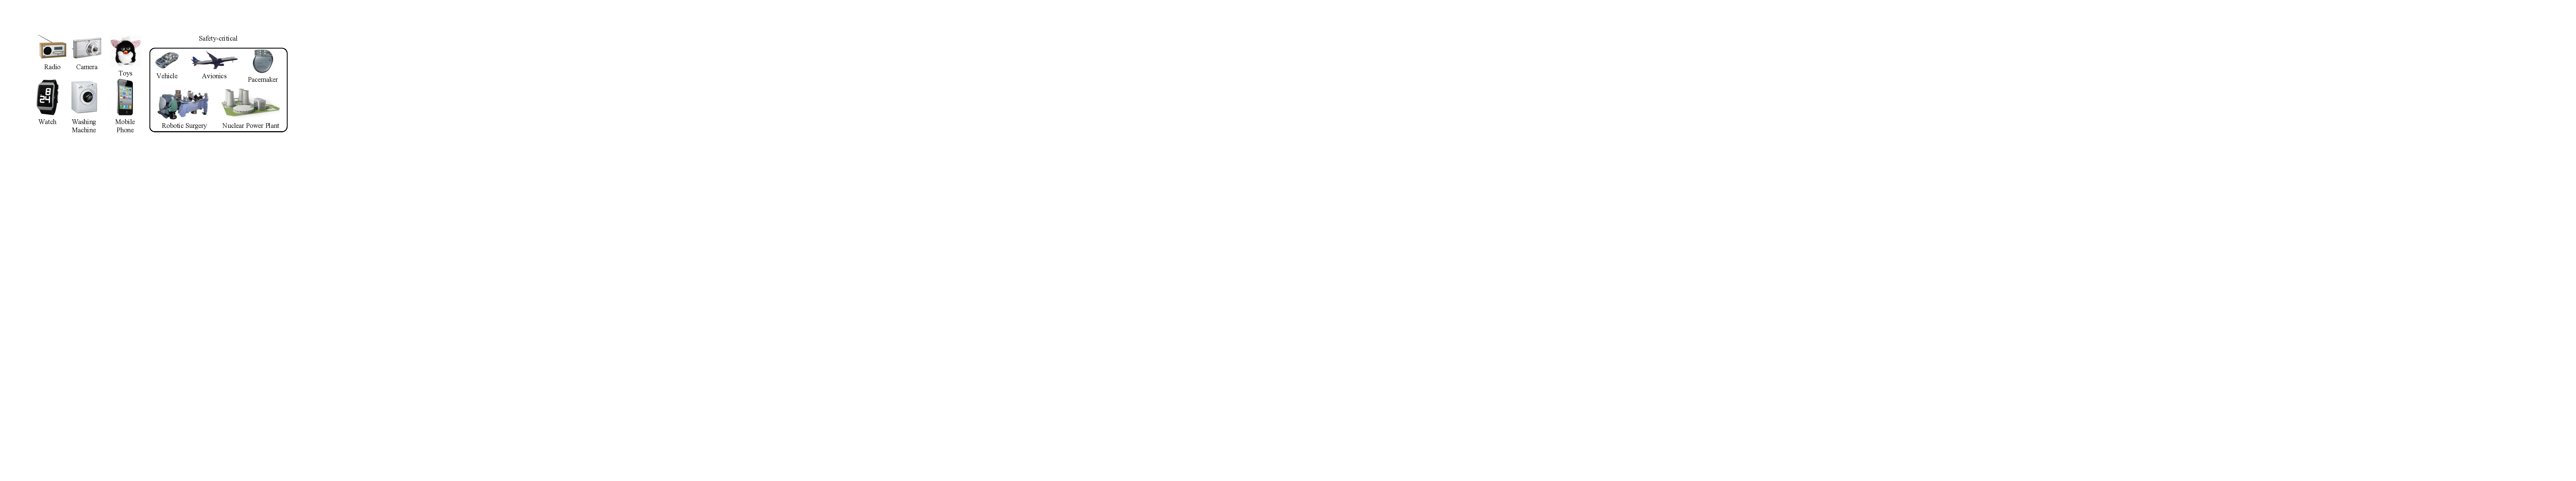
\includegraphics[width=0.9\columnwidth]{embedded_systems}

	\caption{Examples of embedded systems and those with safety-critical concerns.}
	\label{fig:introduction:embedded_systems}
\end{figure}

\subsection{Parallel Programming of Embedded Systems}
\label{sec:introduction:programming}
Programs can be
executed directly by the hardware (bare-metal) or by a
real-time operating system (RTOS)~\cite{pret_merasa_rtos}. 
The bare-metal approach allows all of the system's resources to be used
to execute the program, but code must be included 
to manage the hardware. By contrast, an
RTOS manages the hardware and provides a
consistent environment for developing and executing
programs, thus, enabling code portability across a range of
systems. Hence, the RTOS must be taken into account when analyzing programs. 
C~\cite{programming_languages_c11} is a popular language for 
programming embedded systems with 
support for multi-threading and parallelism 
provided by third-party libraries, compilers, and 
runtime support~\cite{DiazMN12}. Notable 
examples include Pthreads~\cite{multiprocessor_pthreads},
OpenMP~\cite{multiprocessor_openmp}, and
MPI~\cite{multiprocessor_mpi}. 
These multi-threading solutions are inherently
\emph{non-deterministic}~\cite{multiprocessing_problem_threads}
because they allow non-deterministic constructs,
such as race conditions over shared variables in
the case of Pthreads and OpenMP.
The lack of formal semantics for the programming model 
can also lead to ambiguous behaviors. 

Parallel programming is challenging because it requires 
programmers to have specific skills, experience, and 
knowledge to avoid the common parallel programming traps and 
pitfalls~\cite{multiprocessing_debugging_concurrency}. 
For example, parallel accesses to the same shared 
variable will interfere and corrupt the value of the shared variable. 
It is the programmer's responsibility to identify
the regions of code that can interfere, called \emph{critical sections}, 
and ensure that they are executed sequentially at
mutually exclusive times. Hence, programmers need to be 
aware of the data dependencies in their specific program 
and to choose the appropriate solution to manage the dependencies. 
Studies have shown that, without careful tuning~\cite{multithreading_multicore_issues}, 
parallel programs executed on multi-cores can perform 
worse than their sequential counterparts.
The next section describes the use of \emph{synchronous 
languages} as an alternative to creating concurrent programs 
that are deterministic.

\subsection{Synchronous Languages}
\label{sec:introduction:synchronous}

Synchronous languages~\cite{timed_synchronous_survey} 
are based on sound mathematical semantics, which facilitates 
system verification by formal methods~\cite{timed_synchronous_survey} and the
generation of correct-by-construction implementations~\cite{timed_cec,NataleZ12}.
Figure~\ref{fig:introduction:synchronous_moc} depicts a
synchronous program, defined as a set of concurrent threads,
within its physical environment. 
Synchronous programs react continuously to inputs from the environment 
by producing corresponding outputs. Each reaction is triggered by a 
hypothetical (logical) \emph{global clock}. At each global tick, the threads 
in the program sample the environment, perform their computations, and 
emit their results to the environment. When a thread completes its
computation, we say that the thread has completed its
\emph{local tick}. When all threads in the program have
completed their local tick, we say that the program has
completed its \emph{global tick}. Central to synchronous languages 
is the \emph{synchrony hypothesis}~\cite{timed_synchronous_survey}, 
which states that the execution of each reaction is considered to be 
atomic and instantaneous. 
The sampling of inputs avoids the need to use
interrupts which are sources of unpredictable delays that degrade the
system's timing predictability. Concurrent threads
communicate instantaneously with each other (dashed arrows in
Figure~\ref{fig:introduction:synchronous_moc}) due to the
synchrony hypothesis. Once the embedded system is
implemented, the synchrony hypothesis has to be validated.
That is, the worst-case execution time~\cite{wcet_methods_survey} 
of any global tick must not exceed the minimal inter-arrival 
time of the inputs.

\begin{figure}
	\centering
	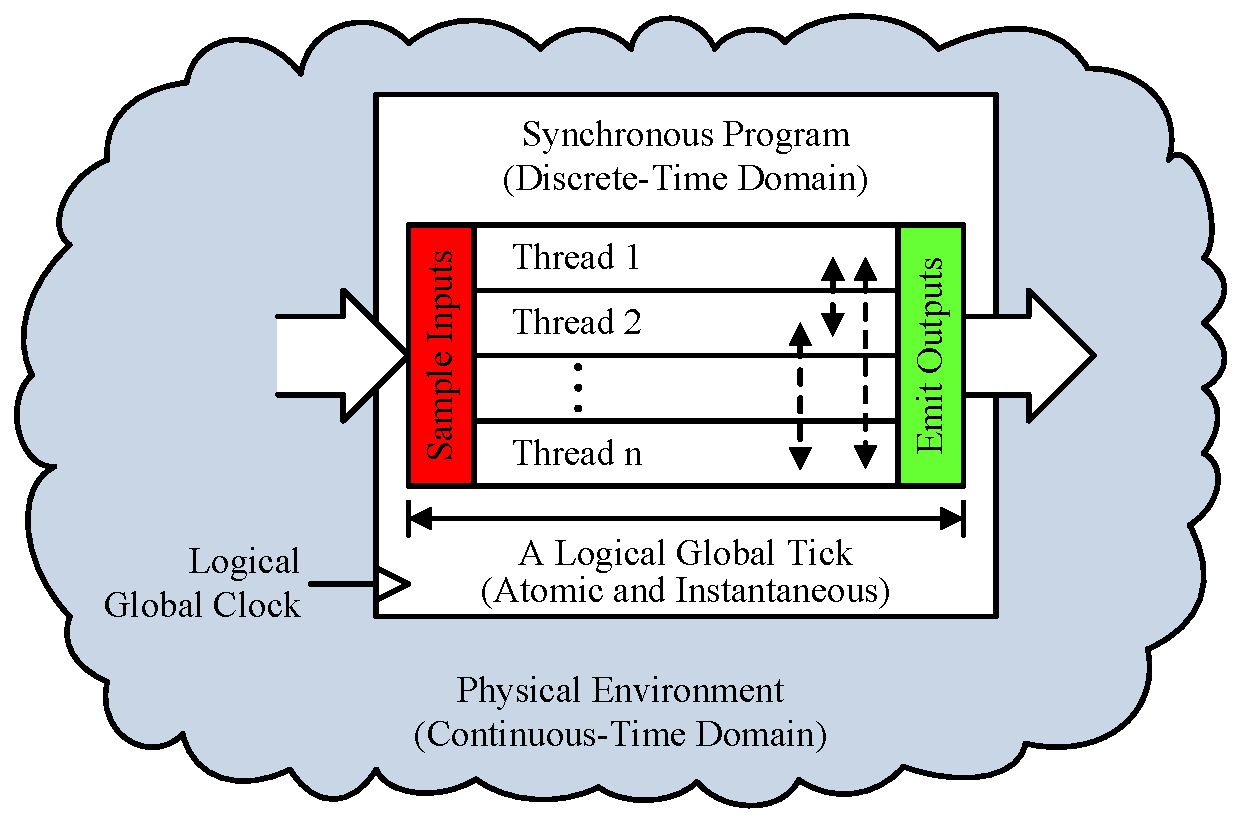
\includegraphics[width=0.8\columnwidth]{synchronous_moc}	

	\caption{Synchronous model of computation.}
	\label{fig:introduction:synchronous_moc}
\end{figure}

\begin{figure}
	\centering

	\subfloat[Esterel]{
		\begin{minipage}[b]{0.4\columnwidth}
			\lstinputlisting[style=full]{./code/Example.strl}
		\end{minipage}
	
		\label{listing:introduction:Example.strl}
	}
	\hfill
	\subfloat[\pretc{}]{
		\begin{minipage}[b]{0.4\columnwidth}
			\lstinputlisting[style=full]{./code/Example.pretc}
		\end{minipage}
		
		\label{listing:introduction:Example.pretc}
	}

	\caption{Examples of synchronous programs.}
\end{figure}

We use the Esterel synchronous language~\cite{timed_esterel}
to illustrate some features of the synchronous paradigm in
Figure~\ref{listing:introduction:Example.strl}. It contains
two threads (starting from lines~\ref{esterel:thread1} and
\ref{esterel:thread2} respectively), scoped between the square brackets
and separated by the parallel operator $\parallel$
(line~\ref{esterel:par}). The parallel operator is
commutative and associative and specifies that both threads
are executed concurrently. The execution of a thread can be
divided over multiple global ticks with the \verb$pause$
statement (e.g., lines~\ref{esterel:pause1},
\ref{esterel:pause2}, and \ref{esterel:pause3}). The
\verb$pause$ statement \emph{pauses} the execution of its enclosing
thread, demarcating the end of the thread's local tick. All
executing threads must pause or terminate to complete the global
tick. Thus, the \verb$pause$ acts as a
synchronization barrier. At the next global tick, the
threads resume from their respective \verb$pause$s. In Esterel, threads
communicate by \emph{emitting} \verb$signal$s and threads can test
for their \emph{presence} or \emph{absence}. For example,
line~\ref{esterel:signal} declares two signals, \verb$A$ and
\verb$B$, that are emitted by the \verb$emit$ statement when
execution reaches lines~\ref{esterel:emit1},
\ref{esterel:emit2}, \ref{esterel:emit3}, and
\ref{esterel:emit4}. An emitted
signal lasts until the global tick ends, becoming absent in
the following global tick unless it is emitted again. Note
that an emitted signal is logically present from the start of the
global tick to ensure that all the threads see the same
signal statuses, even if the \texttt{emit} statement occurs
later in the global tick. In the first global tick, the
first thread emits the signal \verb$A$. At the same time, 
the second thread tests positively for the
presence of \verb$A$ and emits \verb$B$.
Using the \verb$abort$ statement, a body of code can be
\emph{preempted} by the presence of a signal. Preemption provides a
convenient way to model the transitions and states of a
state machine. In the second global tick of the example
program, the second thread enters an \verb$abort$
(line~\ref{esterel:abort}) that preempts its body
(lines~\ref{esterel:abort_body_start}--\ref{esterel:abort_body_end}) 
if \verb$A$ is present.
Because \verb$A$ is not present, the body is not preempted
and \verb$B$ is emitted. Meanwhile, the first thread
terminates because it has reached the end of its body.

Synchronous programs are considerably difficult to 
parallelize~\cite{distributed_reactive_systems_survey,wcrt_esterel_multicores,YuanYR11} 
due to the need to resolve instantaneous thread communication and
associated causality issues. 
At runtime, all potential signal emitters
must be executed before all testers of a signal. 
If this is not possible, then a causality issue arises. 
Thus, concurrency is typically \emph{compiled away} to
produce only sequential code~\cite{timed_cec}. The common approach for
parallelizing synchronous programs is to automatically
parallelize an intermediate representation of the
program~\cite{distributed_reactive_systems_survey,wcrt_esterel_multicores,YuanYR11,multiprocessing_openmp_synchronous}. 
The techniques differ
in the heuristics used to partition the program to achieve
sufficient parallelism. 

Esterel only supports basic data computations and delegates
complex data computations to a host language, for instance C. Consequently, 
C-based synchronous languages have been developed to provide
data handling at the language level. These languages
extend C with a range of synchronous constructs to support
concurrency, preemption, and thread communication. C-based 
synchronous languages appeal to C programmers because the 
learning barrier for synchronous languages is reduced. 
\pretc{}~\cite{pret_pretc} is one such example and
Figure~\ref{listing:introduction:Example.pretc} is the
\pretc{} version of the Esterel example
(Figure~\ref{listing:introduction:Example.strl}). The two
threads (\verb$t0$ and \verb$t1$, defined on
lines~\ref{pretc:t0} and \ref{pretc:t1}) are arguments to
the parallel operator \verb$PAR$ (line~\ref{pretc:par}).
The \verb$EOT$ statement demarcates the end of a thread's
local tick (e.g., lines~\ref{pretc:eot1}, \ref{pretc:eot2},
and \ref{pretc:eot3}). Unlike Esterel, threads in the
\verb$PAR$'s argument are executed in a left-to-right
(static) order. The thread's local tick must be executed
entirely before the next thread can be executed. In the
example program, \verb$t0$ always executes its local tick
before \verb$t1$. In \pretc{}, threads communicate using
globally declared C-variables, not signals. Because
threads are always executed in a static order, the
local ticks always execute in a mutually exclusive manner. 
Hence, threads can safely access shared variables
without needing to use mutual exclusion constructs; all
\pretc{} programs are thread-safe by construction. In
the first global tick of Figure~\ref{listing:introduction:Example.pretc}, 
\verb$t0$ executes first and assigns \verb$1$ to the shared variable
\verb$A$ (line~\ref{pretc:t0_a}). Then, \verb$t1$ executes 
and checks the condition \verb$A==1$, which is \emph{true}, and assigns
\verb$1$ to \verb$B$. \pretc{} does not suffer from causality
issues because global variables are always present and
variables are always accessed sequentially (within a thread and
across threads). \pretc{} supports preemption with the
\verb$abort$ statement but its behavior differs from
Esterel's \verb$abort$. Preemption occurs when the associated
C-condition evaluates to \emph{true}. The condition is
always checked before the \verb$abort$ body is executed. In 
the second global tick of the example program,
\verb$t0$ terminates because it has reached the end of its
body. Then, \verb$t1$ executes and the condition \verb$A==1$
(line~\ref{pretc:abort_cond}) is checked before the
\verb$abort$ body
(lines~\ref{pretc:abort_body_start}--\ref{pretc:abort_body_end}) 
is executed. The condition is \emph{true}, so the body is
preempted. Execution jumps to line~\ref{pretc:abort_body_end} 
and \verb$t1$ terminates. 

Other C-based synchronous languages exist, such as \synchronousc{}~\cite{timed_synccharts_c_proposal}
and Esterel~C Language~\cite{timed_ecl},
and are reviewed in Section~\ref{sec:literature}. 
However, these languages are not designed to take advantage 
of parallel execution. This paper focuses on developing a C-based,
synchronous language for writing parallel programs that
perform well on multi-core processors and are amenable to 
static timing analysis. 

\subsection{Programming Safety-Critical Embedded Systems}
\label{sec:introduction:programming_safety}
Safety-critical embedded systems need to be 
certified against stringent safety standards, such as 
DO-178B~\cite{DO-178B} or IEC 61508~\cite{IEC61508}, before
they can be deployed and used in the field.
Although the C language is popular for programming safety-critical embedded systems, 
its semantics~\cite{programming_languages_c11} includes unspecified 
and undefined behaviors~\cite{safety_critical_coding_traps_pitfalls}. Strict 
coding guidelines~\cite{safety_critical_coding_misrac_standard,safety_critical_coding_power_10,safety_critical_coding_jpl} 
are typically used by safety-critical programmers to help write well 
defined programs that are deterministic, understandable, maintainable, 
and easier to debug~\cite{safety_critical_coding_structure,safety_critical_coding_misrac_overview}. 
The coding guidelines can be grouped into three main areas: 
\begin{description}
	\item[Code clarity] These guidelines suggest a style for writing programs
		  free of ambiguous statements and to structure code for readability. 
		  For example, the use of braces to clarify the nesting of \verb$if$--\verb$else$ statements
		  or the forbidding of \texttt{goto} statements.
		  Code clarity helps static analyzers parse the program and 
		  attain greater analysis precision.
		
	\item[Defensive programming] These guidelines help minimize the use of 
		  unspecified and undefined behaviors, which contribute to
		  non-determinism. For example, the C semantics does not specify 
		  the evaluation order of multiple expressions, e.g.,
		  in function arguments. Thus, function 
		  arguments with side-effects may evaluate to different values 
		  depending on the evaluation order used by the implementation.
		  To ensure deterministic evaluation~\cite{programming_languages_cholera}, 
		  expressions must not contain any assignment operators, e.g., ``\texttt{=}'', 
		  ``\texttt{+=}'', or ``\texttt{++}''. Furthermore, 
		  the sequencing operator ``\texttt{,}'' must not be 
		  used in expressions.
		
	\item[Runtime reliability] These guidelines help prevent runtime errors 
		  from occurring, even when the program is written correctly. 
		  For example, a runtime error occurs when a program requests for 
		  more memory than is available in the implemented system. To prevent
		  it, memory is always allocated statically at the start of the program.
		  Static verification tools, such as Parasoft~\cite{parasoft}, 
		  Polyspace~\cite{polyspace}, and Parallel Lint~\cite{parallel_lint}, 
		  can be used to identify possible runtime defects.
\end{description}


\subsection{Contributions}
We propose the ForeC parallel programming language for simplifying the
deterministic parallel programming of embedded multi-core systems. 
Execution platforms have evolved from 
single-cores to multi-cores. Hence, all the synchronous languages 
designed for the single-core era must be reinvented to address the 
multi-core challenges. To this end, ForeC is a C-based 
synchronous language designed specifically
for the programming of multi-cores. ForeC brings together the formal 
deterministic semantics of synchronous languages and the benefits of 
C's control and data structures. A key innovation is ForeC's shared 
variable semantics that provides thread isolation and deterministic 
thread communication. Moreover, many forms of parallel patterns
can be expressed in ForeC. We show that ForeC programs are reactive and 
deterministic by construction. ForeC can be compiled for direct execution
on embedded multi-cores or for execution by an OS on desktop multi-cores.
Through benchmarking, we demonstrate that ForeC can achieve better parallel 
performance than Esterel and OpenMP, while also being amenable to static 
timing analysis.

\subsection{Paper Organization}
This paper is organized as follows.
Section~\ref{sec:literature} provides a detailed literature review of
parallel and synchronous programming languages.
Section~\ref{sec:architecture_multicore} describes the multi-core architecture
considered by this paper.
Section~\ref{sec:forec} introduces the ForeC language,
defines the formal semantics, and provides
proofs for determinism and reactivity.
Section~\ref{sec:forec_compiling} describes our compilation
approach for generating code that delivers good parallel performance
and that is amenable to static timing analysis.
Section~\ref{sec:forec_benchmarking} presents benchmarking results
for ForeC's performance on multi-cores and the time predictability
of its execution.
Section~\ref{sec:conclusion} concludes the paper.
